\chap{Conclusion}

\section{Summary}


\section{Recommendations to future work}
\subsection{Improve the dataset content}
\subsection{Visualization of the data}
\subsection{Improve the prediction system}
\subsection{System as a service}
This system has been developed with the idea that it could become a "Service system", that is basically a configuration of technology and organizational networks designed to deliver services that satisfy the needs or wants of customers.
Since the prediction system implemented during this work is almost 100\% reusable, it could be used from people for prediction about any kind of data. 

Basically the idea is to create a web application that allows to let you upload your own dataset, choose your own preferences and prediction settings, and then the system will calculate and display prediction of the current values in the future together with the MAPE (Mean Average Percentage Error) to have an idea bout how accurate are the.\\


\begin{figure}[H]
	\centering
        \makebox[\textwidth][c]{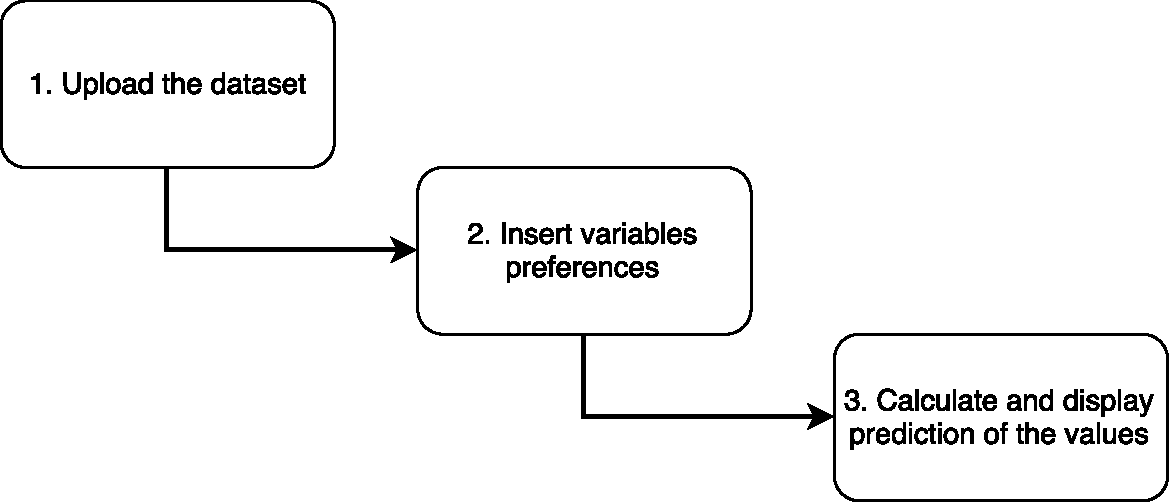
\includegraphics[width=1\textwidth]{Files/ServiceSystem.pdf}}
    \caption{Idea of the Servie System for predictions.}
\end{figure}







